Vyšetřete průběh následujících funkcí:

\begin{enumerate}

	\item  $f(x)=x^3-12x+16$

		\begin{itemize}

			\item  \emph{Definiční obor, průsečíky s osami:}

				\solution{
					$f(x) = x^3-12x+16 = (x-2)^2(x+4)$ je definována pro všechna $x \in \mathbb{R}$.
					Kořeny jsou $2$ (dvojnásobný) a $-4$ a osou $y$ protíná v $f(0)=16$.
				}

			\item  \emph{Limity v krajních bodech:}

				\solution{
					$$\lim_{x \rightarrow \infty} f(x) = \infty$$
					$$\lim_{x \rightarrow -\infty} f(x) = -\infty$$
				}

			\item  \emph{Derivace, monotonie, extrémy:}

				\solution{
					$$f'(x) = 3x^2 - 12 = 3(x - 2)(x + 2)$$ 

					Stacionární body jsou $-2,2$, na intervalech $(-\infty,-2)$ a $(2,\infty)$ je $f'(x)>0$ a tedy $f(x)$ rostoucí, naopak
					na intervalu $(-2, 2)$ je $f'(x)<0$ a $f(x)$ je funkce klesající. 
					Odtud také zjistíme, že v bodě $x=-2$ je lokální maximum a v bodě $x=2$ je lokální minimum.
				}

			\item  \emph{Druhá derivace, konvexita:}

				\solution{
					$$f''(x) = 6x$$
					Inflexní bod pro $x=0$.
					Na intervalu $(-\infty,0)$ je $f''(x) < 0 $ a funkce konkávní,
					na intervalu $(0,\infty)$ je $f''(x)>0$ a funkce $f(x)$ je konvexní.
				}

			\item  \emph{Asymptoty:}

				\solution{
					$$\lim_{x \rightarrow \infty} \frac{f(x)}{x} = \lim_{x \rightarrow -\infty} \frac{f(x)}{x} = \infty$$
					To znamená, že asymptoty neexistují (nemáme směrnice).
				}

				\solution{
					Graf funkce je na Obrázku~\ref{fig:prubeh_fce_a}.
					\begin{figure}[H]
						\centering
						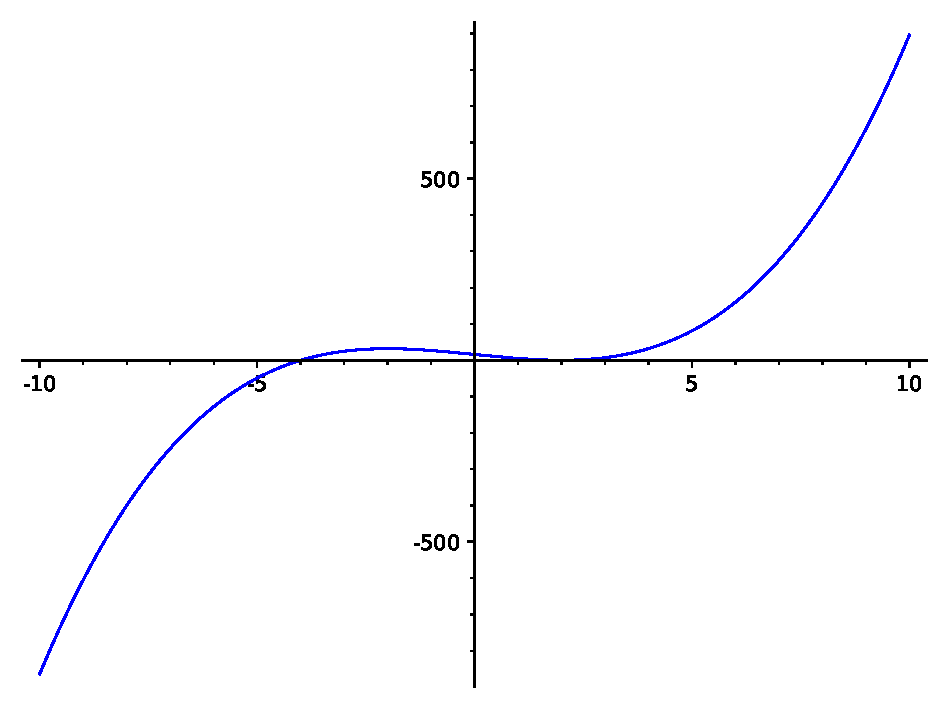
\includegraphics{cviceni_9/fig/prubeh_a.pdf}
						\caption{$f(x) = x^3-12x+16$}
						\label{fig:prubeh_fce_a}
					\end{figure}
				}

		\end{itemize}

	\item  $f(x) = \frac{x^2-1}{x^3-1}$

		\begin{itemize}

			\item  \emph{Definiční obor}

				\solution{
					Funkce $f(x) = \frac{x^2-1}{x^3-1}$ je defnovaná pro všechna reálná čísla vyjma $x=1$.
					$$\lim_{x \rightarrow 1} f(x) = \frac{2}{3}$$
					a lze tak spojitě dodefinovat.

					Uvážím-li $\frac{x^2-1}{x^3-1} = \frac{x+1}{x^2+x+1} = g(x)$ pro $x \neq 1$ a $g(1) = \frac{2}{3}$, je $g(x)$ spojité rozšíření $f(x)$ na celé $\mathbb{R}$.
				}

			\item  \emph{Průsečíky s osami, limity v krajních bodech}

				\solution{
					$$f(0) = 1$$
					Funkce $g(x)$ (a tedy i $f(x)$) má kořen $x=-1$ a
					$$\lim_{x \rightarrow \infty} g(x) = \lim_{x \rightarrow -\infty} g(x) = 0.$$
				}

			\item  \emph{Derivace, monotonnost, extrémy}

				\solution{
					Pro derivaci platí
					$$g'(x) = -\frac{x(x+2)}{(x^2+x+1)^2}.$$
					Ta má kořeny $-2$ a $0$:\\
					Na intervalu $(-\infty,-2)$ je $g'(x)<0$, tedy $g(x)$ je klesající.\\
					Na intervalu $(-2,0)$ je $g'(x)>0$, tedy $g(x)$ je rostoucí.\\
					Na intervalu $(0,\infty)$ je $g'(x)<0$, tedy $g(x)$ je klesající.

					Funkce $g(x)$ má v bodě $-2$ (globální) minimum a v bodě $0$ (globální) maximum.
				}

		\end{itemize}

		\solution{
			Graf funkce je na Obrázku~\ref{fig:prubeh_fce_b}.
			\begin{figure}[H]
				\centering
				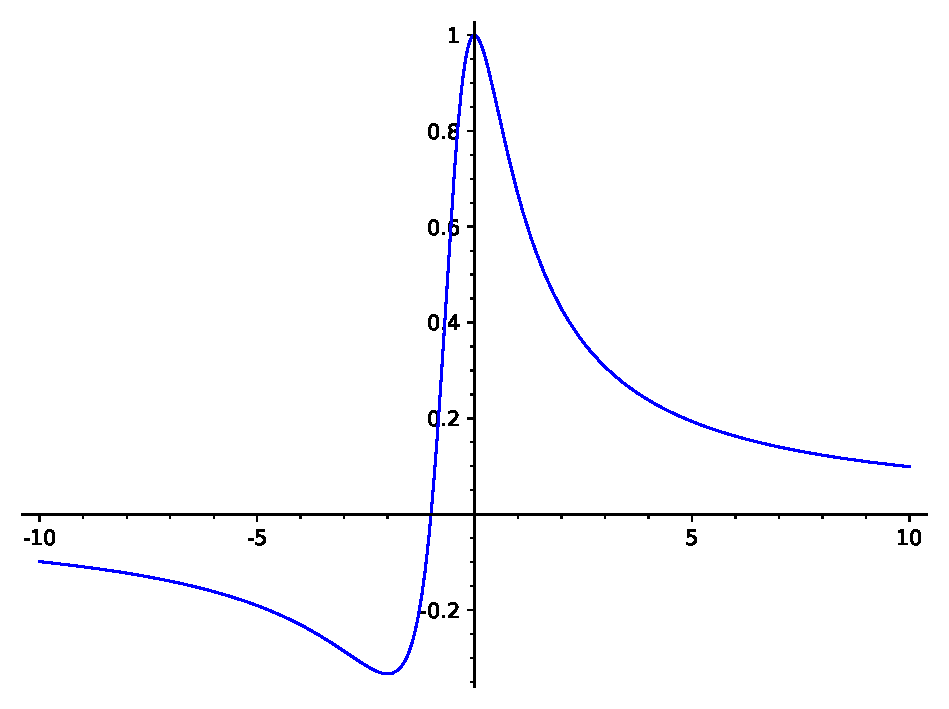
\includegraphics{cviceni_9/fig/prubeh_b.pdf}
				\caption{$f(x) = \frac{x^2-1}{x^3-1}$}
				\label{fig:prubeh_fce_b}
			\end{figure}
		}

\end{enumerate}

